%!TEX program = xelatex
% 完整编译方法 1 pdflatex -> bibtex -> pdflatex -> pdflatex
% 完整编译方法 2: xelatex -> bibtex -> xelatex -> xelatex
\documentclass[lang=cn,11pt]{elegantpaper}

\title{ElegantPaper: 一个优美的 \LaTeX{} 工作论文模板}
\author{\href{https://ddswhu.me/}{邓 东 升}}

\institute{\href{https://elegantlatex.org/}{Elegant\LaTeX{} 项目组}}

% 不需要版本信息,直接注释即可
\version{0.07}
% 不需要时间信息的话,需要把 \today 删除。cn1
\date{\today}


% 如果想修改参考文献样式,请把这行注释掉
\usepackage[authoryear]{gbt7714}  % 国标

\begin{document}

\maketitle

\begin{abstract}
\noindent 本文为 \href{https://github.com/ElegantLaTeX/ElegantPaper/}{ElegantPaper} 的说明文档(中文)。此模板基于 \LaTeX{} 的 article 类,专为工作论文写作而设计。设计这个模板的初衷是让作者不用关心工作论文的格式,专心写作,从而有更加舒适,简便的写作体验。如果你有其他问题、建议或者报告 bug,可以在 \href{https://github.com/ElegantLaTeX/ElegantPaper/issues}{ElegantPaper/issues} 留言。如果你想了解更多由 Elegant\LaTeX{} 项目组设计的模板,请访问 \href{https://github.com/ElegantLaTeX/}{https://github.com/ElegantLaTeX/}。
\keywords{Elegant\LaTeX{},工作论文,模板}
\end{abstract}


\section{模板介绍}

此模板是基于 \LaTeX{} 的标准文类 article设计,也即意味着你可以把 article 文类的选项传递给本模板,比如 \lstinline{a4paper, 10pt} 等等(推荐使用 \lstinline{11pt})。本模板支持 \lstinline{PDFLaTeX} 和 \lstinline{XeLaTeX}\footnote{中文字体均使用 \lstinline{ctex} 包设置。} 两种编译方式。

数学字体的效果如下:

\begin{equation}
(a+3b)^{n} = \sum_{k=0}^{n} C_{n}^{k} a^{n-k} (3b)^k\label{eq:binom}
\end{equation}
      
\subsection{全局选项}
我在这个模板中定义了一个语言选项 \lstinline{lang},可以选择英文模式 \lstinline{lang=en}(默认)或者中文模式 \lstinline{lang=cn}。当选择中文模式时,图表的标题引导词以及参考文献,定理引导词等信息会变成中文。你可以通过下面两种方式来选择语言模式:

\begin{lstlisting}
\documentclass[lang=cn]{elegantpaper} % or
\documentclass{cn}{elegantpaper} 
\end{lstlisting}


\subsection{自定义命令}
在此模板中,并没有修改任何默认的命令或者环境,所以,你可以在此模板使用原来的命令和环境。另外,我自定义了 3 个命令:

\begin{enumerate}
	\item \lstinline{\email}:创建邮箱地址的链接;
	\item \lstinline{\figref}:用法和 \lstinline{\ref} 类似,但是会在插图的标题前添加 <\textbf{图 n}> ;
	\item \lstinline{\tabref}:用法和 \lstinline{\ref} 类似,但是会在表格的标题前添加 <\textbf{表 n}>;
	\item \lstinline{\keywords}:为摘要环境添加关键词。
\end{enumerate}



\subsection{列表环境}
你可以使用列表环境(\lstinline{itemize}、\lstinline{enumerate}、\lstinline{description}),示例如下:\\[2ex]
\begin{minipage}[c]{0.59\linewidth}
\begin{lstlisting}
\begin{itemize}
   \item Routing and resource discovery;
   \item Resilient and scalable networks; 
   \item Distributed storage and search.
\end{itemize}
\end{lstlisting}
\end{minipage}
\begin{minipage}[c]{0.4\linewidth}
\begin{itemize}
   \item Routing and resource discovery;
   \item Resilient and scalable networks;
   \item Distributed storage and search.
\end{itemize}
\end{minipage}




\subsection{插图}
插图的命令和以前一样,也是使用 \lstinline{figure} 环境。\figref{fig:scatter} 显示了插图的效果。你可以把你的图放到当前工作目录的如下子目录下 (\lstinline{./image/}, \lstinline{./img/}, \lstinline{./figure/}, \lstinline{./fig/})。


\begin{lstlisting}
\begin{figure}[htbp]
	\centering
	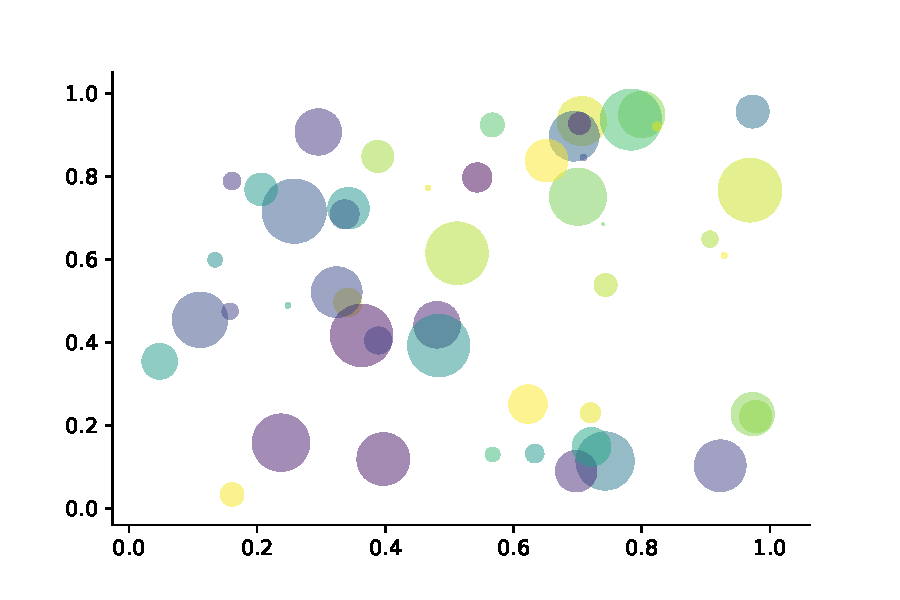
\includegraphics[width=0.6\textwidth]{scatter.pdf}
	\caption{Scatter Plot Example \label{fig:scatter}}
\end{figure}
\end{lstlisting}
\begin{figure}[htbp]
	\centering
	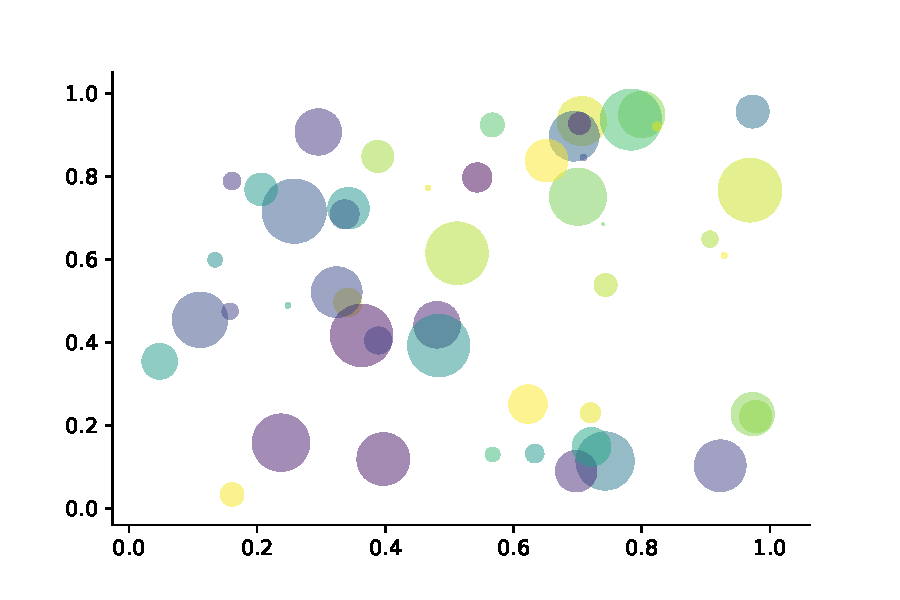
\includegraphics[width=0.6\textwidth]{scatter.pdf}
	\caption{Scatter Plot Example \label{fig:scatter}}
\end{figure}

\subsection{表格}
我强烈建议你使用 \lstinline{booktabs} 宏包,这个宏包有三个命令 \lstinline{\toprule}、\lstinline{\midrule} 和 \lstinline{\bottomrule} 能方便你制作三线表。\tabref{tab:reg} 是一个示例:

\begin{lstlisting}
\begin{table}[htbp]
  \small
  \centering
  \caption{Auto MPG and Price \label{tab:reg}}
    \begin{tabular}{lcc}
    \toprule
                    &       (1)         &        (2)      \\
    \midrule
    mpg             &    -238.90***     &      -49.51     \\
                    &     (53.08)       &      (86.16)    \\
    weight          &                   &      1.75***    \\
                    &                   &      (0.641)    \\
    constant        &     11,253***     &       1,946     \\
                    &     (1,171)       &      (3,597)    \\
    obs             &        74         &         74      \\
    $R^2$           &      0.220        &       0.293     \\
    \bottomrule
    \multicolumn{3}{l}{\scriptsize Standard errors in parentheses} \\
    \multicolumn{3}{l}{\scriptsize *** p<0.01, ** p<0.05, * p<0.1} \\
    \end{tabular}%
\end{table}%
\end{lstlisting}
\begin{table}[htbp]
  \small
  \centering
  \caption{Auto MPG and Price \label{tab:reg}}
    \begin{tabular}{lcc}
    \toprule
                    &       (1)         &        (2)      \\
    \midrule
    mpg             &    -238.90***     &      -49.51     \\
                    &     (53.08)       &      (86.16)    \\
    weight          &                   &      1.75***    \\
                    &                   &      (0.641)    \\
    constant        &     11,253***     &       1,946     \\
                    &     (1,171)       &      (3,597)   \\
    obs             &        74         &         74     \\
    $R^2$           &      0.220        &       0.293    \\
    \bottomrule
    \multicolumn{3}{l}{\scriptsize Standard errors in parentheses} \\
    \multicolumn{3}{l}{\scriptsize *** p<0.01, ** p<0.05, * p<0.1} \\
    \end{tabular}%
\end{table}%



\subsection{参考文献}
此模板使用了 Bib\TeX{} 来生成参考文献,默认使用的文献样式(bib style)是 \lstinline{GB/T 7714-2015}\footnote{通过调用 \href{https://ctan.org/pkg/gbt7714}{\lstinline{gbt7714}} 宏包}。参考文献示例:~\cite{en3} 使用了中国一个大型的 P2P 平台(人人贷)的数据来检验男性投资者和女性投资者在投资表现上是否有显著差异。

你可以在谷歌学术,Mendeley,Endnote 中获得文献条目(bib item),然后把它们添加到 \lstinline{wpref.bib} 中。在文中引用的时候,引用它们的键值(bib key)即可。注意需要在编译的过程中添加 Bib\TeX{} 编译。如果你想在参考文献中添加未引用的文献(部分或者全部),可以使用

\begin{lstlisting}
\nocite{EINAV2010, Havrylchyk2018} % add the two reference.
\nocite{*}   % add all the reference in the bib file.
\end{lstlisting}

如果你想修改参考文献的样式(比如改为 \lstinline{aer}),你可以在导言区将下面代码注释掉。
\begin{lstlisting}
\usepackage[authoryear]{gbt7714}
\end{lstlisting}

并且文档末尾添加

\begin{lstlisting}
\bibliographystyle{aer}
\end{lstlisting}

\section{示例}
在这部分,我提供一个示例文档:


\begin{lstlisting}
\documentclass[lang=cn]{elegantpaper}

% title information
\title{A Working Paper Example}
\author{ddswhu} 
\institute{Elegant\LaTeX{} Group}
\version{1.00}
\date{\today}

\begin{document}

\maketitle

\begin{abstract}
Your abstract goes here.
\keywords{keyword1, keyword2}
\end{abstract}

\section{Introduction}
The content of introduction section.

\section{Conclusion}
The content of conclusion section.

% include the noncited reference
\nocite{ref1, ref2}
\bibliographystyle{aer}
\bibliography{wpref}
\end{document}
\end{lstlisting}

\nocite{*}

% 如果想修改参考文献样式(非国标),请把下行取消注释,并换成合适的样式(比如 unsrt,plain 样式)。
%\bibliographystyle{aer}
\bibliography{wpref}

\end{document}
